%*----------- SLIDE -------------------------------------------------------------
\begin{frame}[c]{Método BiLi}
    %\transboxin[duration=1,direction=30]
    \begin{figure}
        \centering
        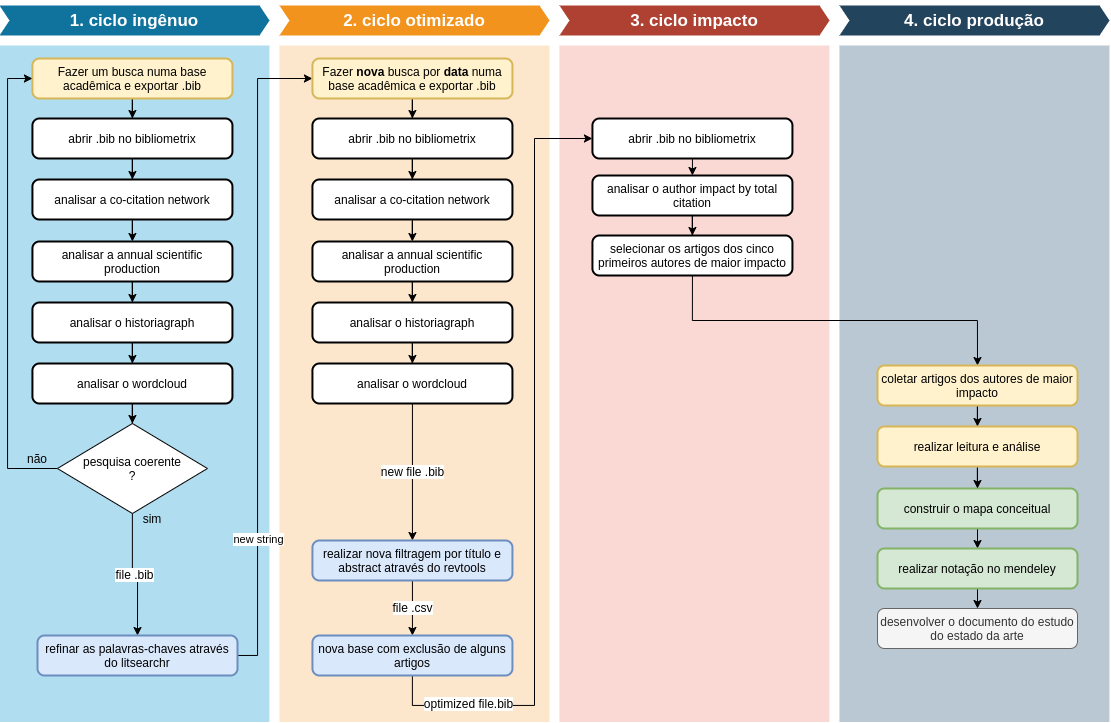
\includegraphics[width=0.7\textwidth]{bili-fluxograma.png}
    \end{figure}
%*----------- notes
    \note[item]{Notes can help you to remember important information. Turn on the notes option.}
\end{frame}
%-

%*----------- SLIDE -------------------------------------------------------------
\begin{frame}[c]{Mapa de Palavras}
    \framesubtitle{Ciclo Ingênuo X Ciclo Otimizado}
    %\transboxin[duration=1,direction=30]
    \begin{figure}
        \centering
        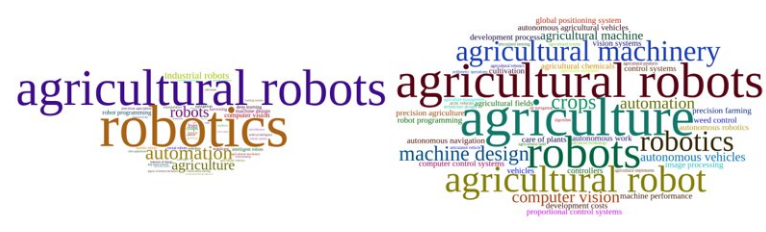
\includegraphics[width=1\textwidth]{bili-wordclould.png}
    \end{figure}
%*----------- notes
    \note[item]{Notes can help you to remember important information. Turn on the notes option.}
\end{frame}
%-

%*----------- SLIDE -------------------------------------------------------------
\begin{frame}[c]{Evolução Temática}
    %\transboxin[duration=1,direction=30]
    O tema de pesquisa apresentou \textbf{crescimento anual} de produção científica de \textbf{10,76\%} (2016 - 2021)\\
    \begin{figure}
        \centering
        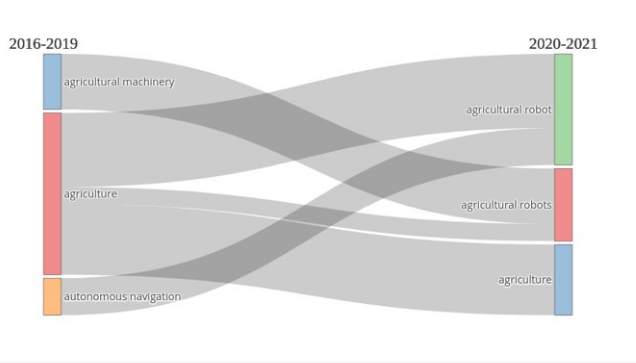
\includegraphics[width=0.65\textwidth]{bili-thematic-evolution.png}
    \end{figure}
%*----------- notes
    \note[item]{Notes can help you to remember important information. Turn on the notes option.}
\end{frame}
%-

%*----------- SLIDE -------------------------------------------------------------
\begin{frame}[c]{Referencial Teórico}
    A tabela abaixo apresenta 4 dos 8 artigos que serão empregados ao longo do estudo do estado da arte
    \begin{table}
        \centering
        \begin{tabular}{cc} 
        \hline
        \textbf{TEMA} & \textbf{AUTOR(ES)}                                                                        \\ 
        \hline
        \begin{tabular}[c]{@{}c@{}}Veículo autônomo com navegação de precisão\\para supervisão de plantações\end{tabular}  & \cite{Xue2010} \\ 
        \hline
        \begin{tabular}[c]{@{}c@{}}veículo autônomo\\semeador\end{tabular}  & \cite{Santhi2018}  \\ 
        \hline
        \begin{tabular}[c]{@{}c@{}}visão computacional para classificação\\de cultivos e ervas daninhas\end{tabular}  & \cite{Jasiski2018} \\ 
        \hline
        \begin{tabular}[c]{@{}c@{}}sistema autônomo para plantio\\e colheita\end{tabular}  & \cite{Munch2019} \\                                           
        \hline
    \end{tabular}
    \end{table}
        
%*----------- notes
    \note[item]{Notes can help you to remember important information. Turn on the notes option.}
\end{frame}
%-